 \documentclass[11pt,letterpaper]{article}
\usepackage[applemac]{inputenc}
\usepackage{graphicx} 
\usepackage{html}
\usepackage{rotating}
\author{David Reitter and Kevin Walzer}
\title{Aquamacs User Help}
\begin{document}
\maketitle

\tableofcontents
\pagebreak



\section{Emacs: The Aquamacs Distribution}

Aquamacs is an freely-available Aqua-native build of the powerful Emacs text editor (\url{http://www.gnu.org/software/emacs/emacs.html}). By ``Aqua-native,'' we mean more than just the fact that this version of Emacs runs as a standard OS X application. Aquamacs features extensive customization that enables it to conform better with Apple's standard Human Interface Guidelines (HIG) than standard versions of the editor do. 

Emacs is a text editor of legendary power and configurability, but it also has an enormously complex interface that, while consistent across platforms, is usually at odds with the specific interface conventions of the particular platform on which it is being used. The official OS X version of Emacs, called Carbon Emacs, is no different. 

The Aquamacs distribution implements the standard OS X keyboard
shortcuts and other interface conventions, integrating Emacs into the
Aqua environment to a far greater degree than other versions of
Emacs. This allows Mac users who might be unfamiliar with Emacs'
complex standard interface to harness its amazing editing power in a
familiar way. 


\begin{figure}
\centering
{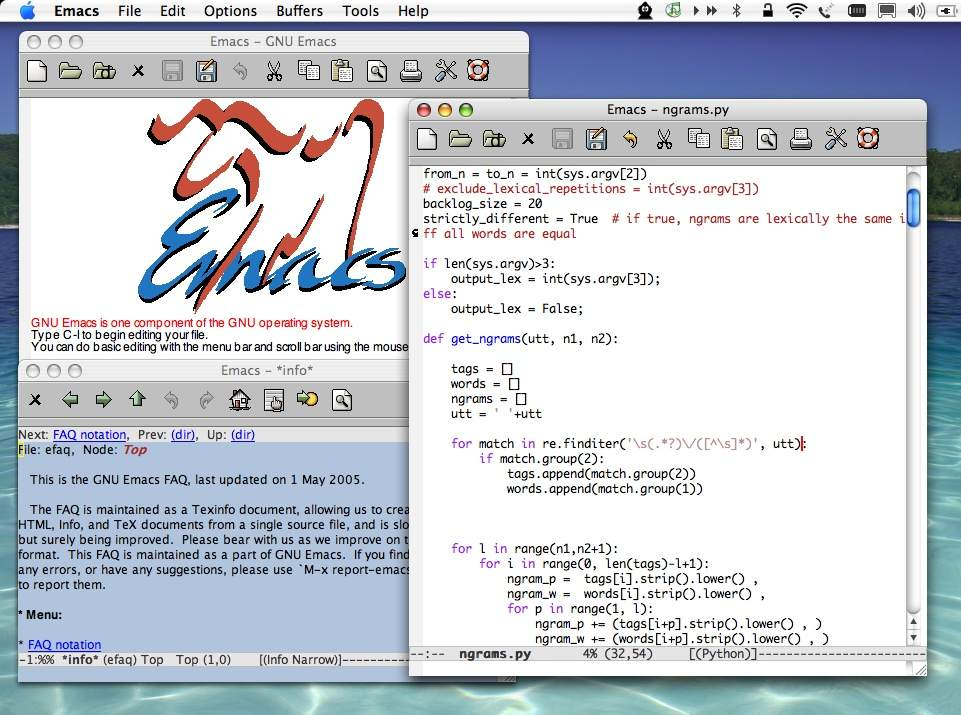
\includegraphics[width=5in]{aquamacs-screenshot.jpg}}
\caption{Aquamacs combines the legendary power of Emacs with
  user-friendly customizations to provide a more Aqua-specific user experience.}
\label{aquamacs-screenshot.jpg}
\end{figure}

You can always download the latest version of Aquamacs from the
project home page, \url{http://www.aquamacs.org}. The direct download link is \url{http://aquamacs.org/cgi-bin/download.cgi}. Just
download the disk image (DMG), move the Aquamacs application bundle to
your hard drive, and launch.  


This documentation aims to introduce Aquamacs to novice users of
Emacs, to help them get started with this powerful text editor. The
documentation also aims to introduce Aquamacs to experienced users of
Emacs, who may find aspects of its interface inconsistent with their
experience.

The Aquamacs documentation will focus on the following areas:

\begin{itemize}
\item What's New in this Release
\item Tutorial: Aquamacs for Beginners
\item In-Depth: The Aquamacs Interface
\item Aquamacs for Emacs Veterans
\end{itemize}

Our hope is that using Aquamacs will be a rewarding experience both
for new users, who come to appreciate the power of Emacs without the
steep learning curve, and for experienced Emacs users, who may find
Emacs' integration into the Aqua environment an unexpectedly
pleasant surprise.

\section{What's New in This Release}

This is version 0.9.4 of Aquamacs, released July 2, 2005. Aquamacs 0.9.4 is a bugfix release; it corrects a number of issues  that occurred in 0.9.3.
As a result of one bugfix, you may notice a change in font size.  Please adjust your font settings to accomodate for that. 


\subsection{New Download Location}

The latest version of Aquamacs can always be dowloaded at \url{http://aquamacs.org/cgi-bin/download.cgi}. 


\subsection{Bug Fixes---0.9.4}

\begin{itemize}
\item Bug reports contain the subject line that the user entered.

\item No more (delay due to) tramp mode on startup in cases where tramp
    mode had been used before (recentf).

\item Files on externally mounted volumes aren't checked for readability
    any more for exclusion from recent files list.
    (Reported by Bill Clementson)

\item No more warnings when fonts are missing (on startup).

\item Drag and Drop while in minibuffer works again.

\item Mouse-2 works again.

\item default-major-mode and initial-major-mode are respected now.
    initial-frame-alist is not modified any more.
    Note that other than in any standard Emacs, mode-specific settings
    always take precedence over default-frame-alist (but not over
    initial-frame-alist).
    (Reported by Rick Zaccone, Joe Davison and Peter Dyballa)

\item No more warnings in customization buffers that the values have
    been changed outside customize (for certain variables).

\item Gnus articles (newsreader) open in same frame now.

\item Gnus has a useful (free) nntp server set so you can start right
    away.

\item Send Email with Sendmail is gone from menu (doesn't usually work
    on  OS X).

\item Fonts corrected: Some glyphs in some fonts turned out wrong when
    in bold or italic. Also, font sizes are correct again (Lucida 14
    is Lucida Grande 14, not 12 or so). The default font size for
    text-mode (and similar ones) is set to Lucida 13 to make up for
    the change.  Apologies for any inconvenience this may cause with
    your default settings. (Reported by William Henney)

\item Better customization for aquamacs-mode-specific-default-themes

\item The customizations file (customizations.el) doesn't grow any more.
    (Reported by Alastair Rankine.)

\item Various corrections in the Aquamacs Manual.

\item Plugin support: All files named site-start.el anywhere in the load-path
    are loaded at startup, before the user's init files are
    loaded. For example, such a file may be placed in
    ~/Library/Application Support/Aquamacs Emacs/myPlugin. This
    feature enables support for easily installable plugins.

\item We anticipate shorter startup times in the next release. Stay tuned.
\end{itemize}


\subsection{Bug Fixes---0.9.3a and 0.9.3b}

\begin{itemize}

\item Fixed ``wrong argument type" problem (version check),
    which could occur in new installations or those updated from 0.9.1.

\item Monaco 18 font present (suggestion: David M. Cook).

\item Emacs Manual available again.

\item Save mac-pass-option-to-system when saving options.
\end {itemize}


\subsection{Bug Fixes---0.9.3}

\begin{itemize}

\item Initial-frame-alist is respected. (Reported by Alastair Rankine)


\item When saving a buffer and the Finder is not running, 
	the Finder is not opened any more. (Reported by George W. Gilchrist.)

\item Using dead-keys (like Option-u or Option-n on most
	keyboards) works again. (Reported by Howard Melman and Pierre Albarede
\item When modified files existed, but no frame was visible and
    one tried to quit Aquamacs, the application seemed to hang while
    prompting for keyboard input (Save file? y/n) in an invisible
    window. This has been fixed. 

\item If no frame is visible and you input text, the frame is  made
    visible so you can see what you are doing.

\item Closing windows consistently with the mouse now works properly. 

\item Clicking on links to source files in help buffers properly
    opens a new frame (if ``open buffers in separate frames" is on).

\item When the buffer shown in a frame changes, sometimes the
    color theme and font were not set correctly; this has been addressed. This could happen when
    ``Show Buffers in Separate Frames'' was off, and one killed a
    buffer. (Reported by Peter Dyballa.)

\item When ``Show Buffers in Separate Frames'' was off, and one killed a
    buffer (kill-buffer, C-x k), the frame was deleted.

\item You have the option to save newly created buffers (Command-N)
    that have not been saved yet when you quit Aquamacs.

\item Less frame-dancing (resizing) on startup.

\item AUC\TeX\ uses the standard commands again. The menu is
  unstructured for this reason. (Reported by Robert Sloan.)

\item No frames could be opened when using a two-screen setup
    with the menu bar on the right screen, and a currently selected
    frame on the left screen. This has been addressed.  (Reported by George W. Gilchrist.)

\item Customizing a theme for a special display frame (e.g.  help or
    customization) works now.

\item Recent Files/Clear Menu works again.

\item Paths and other environment variables are now derived
    from the shell  when
    you start Aquamacs. 



\item Your settings for highlight parens,``Blinking Cursor," etc.  are now
    persistent. The function Options/Save Options
    (menu-bar-option-save) now correctly saves such settings. This
    should include most customization settings except some that
    Aquamacs relies on for proper clipboard copy/paste functionality.

\item The font menu (Options) no longer includes non-existent fonts. 

\item Option/Show-Hide/Menu Bar is gone because you cannot turn off  the
    menu bar on OS X.

\item ``Send Emacs Bug Report'' now uses the OS X
    default mail program to compose
    a message. This ensures that bug reports actually go through.
    Before, they did not, unless you were running a local SMTP server
    (sendmail/postfix), which is not enabled by default.

\item Fixed loading of files when file names contain certain  Kanji characters,
    due to a bug in AppleScript.

\item The menu shortcut entries were corrected.

\item Characters that require the use of the option key work again. For
    example, Alt-3 produces the pound sign (�) on a US keyboard,
    Alt-L the `at' sign @ and Alt-Shift-7 the backslash \ on a
    German one. Inputting the Euro sign works, too. However, that means that the option key is not used to emulate
    the `meta' modifier;  you will have to use Esc to do that.
    Alternatively, you can map the option key to meta in your .emacs
    file:

\texttt{    (setq mac-option-modifier 'meta)}

	 \item Improvements in the fontset selection allow you to display the  Euro sign
    with the default font.
    
    \end{itemize}


\subsection{Features and Changes: 0.9.3}

\subsubsection{New Address}

\begin{itemize} 

\item We have moved Aquamacs to \url{http://www.aquamacs.org}.

\item The Aquamacs wiki is now at \url{http://www.emacswiki.org/cgi-bin/wiki/AquamacsEmacs/}.

\item The Aquamacs bug reporting address is now \url{mailto:aquamacs-bugs@aquamacs.org}. This can be accessed from directly within the Aquamacs Help menu.

\item The general Aquamacs mailing list is still \url{mailto:macosx-emacs@email.esm.psu.edu}; e-mail \url{mailto:macosx-emacs-on@email.esm.psu.edu} to subscribe.

\end{itemize}

\subsubsection{Running Aquamacs}
	
\begin{itemize}

\item Slightly faster startup.

\item Runs on OS X 10.3.9, 10.4.0 and 10.4.---tested.

\item Aquamacs automatically checks for updates and notifies the user
    if there is something new. This function communicates with an internet server; it does not
    transmit any information identifying the user. If you would like to
    know more about what is transmitted, use M-x
    aquamacs-check-version-information. If you like to turn this check off, add this to your file
 /Users/ yourname / Library /Preferences /Aquamacs Emacs/ Preferences.el:

    \texttt{(setq aquamacs-version-check-url nil)}

\item Adding Emacs packages is easier now: Emacs automatically finds
    packages in subdirectories within the /Library/{Preferences| Application
    Support}/{Emacs|Aquamacs Emacs}/ paths.

\item Aquamacs now sets the file creator information of files it
    writes. This helps to open the file from Finder with Aquamacs when
    you double-click it. Feature can be turned off via customization
    option ``aquamacs-set-creator-codes-after-writing-files.''  Also,
    Emacs will appear in the Finder's context menu under ``Open With''
    for a lot of files that it is commonly used to edit.

\item You can start Aquamacs in a terminal (by running
    /Applications/ Emacs.app /Contents/ MacOS/ Emacs) with parameter -nw
    and will show up in the terminal rather than as a  Carbon
    application. Basic file editing and all traditional commands
    work. However, Aquamacs-specific keyboard commands (with the
    Command key) will not work and other functionality may be limited,
    too. \textit{Warning: }This mode of use, which may break in future versions, is not
    supported by the Aquamacs team.
    \end{itemize}
	
\subsubsection{Frame and Window Operations}
	
We make sure that the *Completions* buffer (and similar things)
    open as a window inside the frame directly above the Minibuffer,
    and not in a new frame.

All newly opened frames open in a somewhat useful position, so
they are not in the way. (If you do not like this, we suggest you set
    your own static frame positions via ``set current theme as default''
    and also add this to your file / Users / yourname / Library / Preferences/ Aquamacs
    Emacs/ Preferences.el:

	\texttt{ (setq smart-frame-positioning-enforce nil)}

Or, if you would like to go with the default position all the time,
    turn the global minor mode off:

   \texttt{(smart-frame-positioning-mode nil)}


\subsubsection{Fonts}
	
\begin{itemize}
	
\item Aquamacs should not complain about missing fonts any more when
    you have upgraded from earlier versions and set scalable fonts as
    default fonts for modes or all frames. They get filtered  automatically.

\item Users with certain setups (cyrillic Lucida Grande) should not get
    a ``default font not found'' error any more.

\end{itemize}

\subsubsection{Interface}

\begin{itemize}

\item ``Recursive Minibuffers'' are enabled. 

\item ``Subscribe to mailing list'' in Help menu.

\item PHP-Mode included (M-x php-mode).

\item Ruby-Mode included (M-x ruby-mode)

\item yes-or-no-p is customizable now. Use the new customization
 	variable aquamacs-quick-yes-or-no-prompt. (Thanks: Pavel Hlavnicka.)

\item Soft word wrap (longlines-mode) is available from the Options
	menu. To make it the default, add this to your preferences
	file:	
	\texttt{(set-default 'longlines-mode t)}

\item Case-insensitive search option has gone into ``search'' submenu (in ``Edit'').

\item If you are in an empty frame (i.e. a frame with an empty buffer)
	and you load (find) a file, Aquamacs will not open an additional frame.
	This is useful also for drag and drops, when a scratch frame is open.

\item The secondary selection is back: use the Command (Apple) key
    together with clicking/dragging the mouse cursor over text in
    order to select text that is not related to the point
    (cursor). This way, you can select text and then scroll somewhere
    else. Extend your selection with shift-command-mouse1.
    To copy/cut the text in the secondary selection to the  clipboard, use
    Shift-Command-C/X, respectively.

\item Some key-bindings are more like the original Emacs ones--in
    particular M-w, which does kill-ring-save again.
    (Idea: Joe Davison)   Also, Home and End keys work as expected.

\item No more annoying system ``ding'' (bell ringing) all the time.  The bell is
    turned off completely, until Emacs developers eliminate the use of
    the bell on user-initiated abort actions (such as ESC ESC ESC when
    in minibuffer, of pressing Cancel in the file selection dialog).
	
\item The toolbar is only displayed in normal frames, but not
    in frames that show help/info buffers. (tool-bar+ and
    aquamacs-tool-bar packages). Turn such toolbars on/off in
    Options/Show/Hide menu.
	
\item The ``About Emacs'' dialogue has been improved.

\item Key combinations with the option key that  involve
    another modifier (that is, ctrl or command) will now work, even
    though simple option combinations are handled by the system to
    produce special characters.

\item The Speedbar is back. Activate in Options/ Show/Hide.

\item The redo function is in the Edit menu now.

\item New buffers (File / New) open in Text Adapt Fill mode now.

\item .save-places and customizations.el do not show up in the recent  files list
    any more.

\item auto-save-files (in / Users / yourname /.emacs.d) are now saved to / Users / yourname/Library/Preferences.

\item ``Save Place in Files in between sessions'' will not generate  files in the
    user's home folder any more. Instead, the file goes into
    / Users / yourname/Library/Preferences/Aquamacs Emacs/ where it belongs.

\item Command-' now cycles between different windows (suggested  by Joseph Kiniry.)



\item Option is mapped to Meta by default, allowing you to enter key
    combinations such as C-M-\ easily. If you'd like to map it to
    alt instead, just add this to your .emacs:

   \texttt{(setq mac-option-modifier 'alt)}

\end{itemize}


\subsubsection{Configuration}

\begin{itemize}

\item Color Themes: The color-themes package has been integrated in
    Aquamacs. Use the Option/Color Theme... menu command to choose a
    set of predefined colors for editing source code or writing
    texts. This applies to the current frame only, but you can make it
    the default for all new frames or for all frames in a specific
    mode with the according menu commands.

\item There is a new customization group called ``Aquamacs'' that
    allows you to modify the customizations introduced by Aquamacs.
    This is fairly untested - unexpected results may occur. If so, try
    to locate and fix the bug and send us a patch. If you couldn't
    find the problem, please report via Help/Send Bug Report...
    PLEASE NOTE that a lot of customization variables have changed
    their names---usually, you just need to prepend 1on1  to them.

\item Aquamacs will load YOUR configuration files not just from
    / Users / yourname/.emacs, but also from the location that is appropriate for a Mac
    OS X installation:

/ Library/ Preferences /Aquamacs Emacs / Preferences.el\\
/ Users / yourname/Library/Preferences/Aquamacs Emacs/Preferences.el\\
  /Library/Preferences / Emacs / Preferences.el\\
 / Users / yourname / Library/Preferences/Emacs/Preferences.el\\



    It is recommended to use these instead of / Users / yourname/.emacs on OS X-only
    installations. The first two files should be used for the
    host-wide and user-specific Aquamacs configs, the latter two for
    general Emacs configurations.

\item There is a new configuration option that gives you more fine-grained
    control over how the option modifier key is handled.

\item If mac-pass-option-to system is nil, your Aquamacs will get all key
    combinations. If you press option-3, Aquamacs will see ``M-3'' (or,
    depending on mac-option-modifier ``A-3''). If it is non-nil, you
    will simply get the pound sign (�) on a US keyboard.

\end {itemize}

\subsubsection{External Tools Support}

\begin {itemize}

\item TeXniScope support in LaTeX mode (if installed in /Applications).

	\end{itemize}

\subsubsection{User Documentation}

	
\begin{itemize}

	\item We have two great manuals available comfortably via Apple Help  now,
    directly from within Aquamacs Emacs (Help menu). There is a
    brand-new Aquamacs manual, and there is Richard
    Stallman's original Emacs manual. They can be searched (e.g. via
    Spotlight on OS X 10.4). We also provide direct access to the online configuration Wiki, which has been filling up with content nicely.  Please contribute; everybody has write access!
	\end{itemize}



\section{Tutorial: Aquamacs for Beginners}

\subsection{What Makes Aquamacs Like Other Text Editors} 
When you first launch Aquamacs, you will see that it is like many
other text editors such as Bare Bones Edit, Dreamweaver, or similar programs: you can type text, cut and paste text, and save
and close a file using the menubar or standard OS X keyboard shortcuts
(Apple-S for save, Apple-X for cut, Apple-V for paste, and so on). If you are writing one of the many text formats that
is supported by Aquamacs, such as HTML, you will also note Aquamacs'
use of \textit{syntax coloring,} which sets certain parts of the
text---such as HTML markup---in a different color than the text
content. This makes editing the text and adjusting the markup easier.

\subsection{What Makes Aquamacs (Emacs) Different from Other Text
  Editors}
If you look at some of the menu items and keyboard shortcuts, you will
see some of the features that make Emacs different from other text
editors. Although Aquamacs has been designed to present many of these
features in an Aqua-friendly way, it does not hide these
features. Aquamacs is a complete editing environment.

\begin{itemize}

\item \textbf{Sophisticated text processing.} Aquamacs features text
  editing capabilities that go far beyond the average text editor. For
  instance, Aquamacs features several kinds of search and replace: it
  can replace text incrementally, it can search and replace text by
  complex patterns of characters (regular expressions) and not just by
  word matching, and so on. Aquamacs also features support for
  virtually every kind of text file imaginable: computer code such as
  C/C++, HTML, \LaTeX, XML, and other formats. 
\item \textbf{The buffer.} One of the features that makes Emacs such a productive editing
environment for experienced users is the \textit{buffer.} The buffer
includes any window in which text is being edited, similar to a
standard Aqua ``Document'' window, but also includes windows
that display messages from the program, a window that you can use to
actually send commands that Aquamacs executes, and other functions. The
buffer feature of Aquamacs allows you to switch quickly between
windows, to send execute or preview the code you are writing with a
couple of keystrokes, and to monitor logs of commands you are
executing. You can also split a single window into multiple buffer
displays if you choose.
\item \textbf{Integration with additional tools.} Aquamacs' ``Tools''
  menu provides access to file comparison and version control,
  compiling and debugging of program code, the ability to read e-mail
  and newsgroups, and more.

\end{itemize}

In addition to its large number of features, Aquamacs also defines
some interface terms differently than other OS X applications. See
Table \ref{tab:terms} for more information.


\begin{table}[t]
\begin{center}
\begin{tabular}{|c|c|}
\hline  OS X Term & Emacs Term  \\ 
\hline  Window &  Frame \\ 
\hline  Tab/pane  &  Window \\ 
\hline Document &  Buffer \\ 
\hline Keyboard shortcut &  Key \\ 
\hline 
\end{tabular} 
\caption{Key Emacs terms and their Apple counterparts.}
\label{tab:terms}
\end{center}
\end{table}

This list provides just a small sampling of the functionality
available in Emacs. Aquamacs' customizations make Emacs much easier to
learn; it is possible to get started and become productive
quickly. However, harnessing all of Emacs' power, even with assistance
from the Aqua shortcuts, will take time.



\section{In Depth: The Aquamacs Interface}

In this section, we will walk through the Aquamacs interface step by
step, and will introduce relevant points about how Emacs solves
particular editing problems in a distinctive way. Here our discussion
will focus on how Aquamacs is configured, as opposed to Emacs in
general.

\subsection{File}
The File menu includes basic operations for opening, closing, and
printing files. Opening and saving files uses standard Mac keyboard
shortcuts (Apple-O, Apple-S), and uses standard Aqua dialog boxes. You
can also open a directory; from the menubar this brings up a standard
Aqua dialog box, through the keyboard shortcuts are the traditional
Emacs one  (control-x d), and it brings up a directory name in the
``minibuffer'' (small space for commands at the bottom of the main
window, or frame). 

Printing is supported, though only from the menu, and it will not
present a traditional Mac print dialog. Instead the text in your file
will print to your default printer using the command-line \texttt{lpr} program.

From the File menu, you can also open a new ``frame,'' or window, or
split the open window into two separate buffers. The keyboard
shortcuts for these commands are the traditional Emacs ones (see the menubar).

\subsection{Edit}
The Edit menu is the heart of Emacs' textual wizardry. Emacs supports
all customary editing functions, such as cut, copy, paste, and simple
search and replace. In Aquamacs these basic functions are supported by
standard Aqua keyboard shortcuts. There is a great deal more
functionality, however, than the average text editor. For instance,
Emacs allows you to go to a specific line number in the file you are
editing, to the top or bottom of the buffer, and so on. It also supports searches with \textit{regular expressions,}
which are sophisticated text patterns that go beyond simply matching a
specific set of characters (or ``string''). Emacs also stores more
than twenty of the most recently-copied items on the clipboard, and
these are accessible from the menu in case you need to paste these
items again.  The Edit menu also supports ``bookmarks,'' a feature
that allows you to save your place in a specific file. 


\subsection{Options}
The Options menu is where you can easily customize your
settings. The options that you can configure include syntax coloring,
matching of parentheses (useful for text markup that depends on open
and close brackets), how to display buffers and frames, color theme, fonts, and other
settings. If you change a setting, such as the color theme or fonts, be sure to
select the ``Save Options'' item in the menu. The changes will not be
saved by default.

\subsection{Buffers}
The Buffers menu allows you to navigate through the windows/frames
that you may have open. Note that a ``buffer'' is not synonymous with
a window or frame, in that you can split a frame and have more than
one buffer contained within. (Multiple windows/frames is a feature of
Aquamacs; standard Emacs does not support this.) In addition to
standard frames that display open files, there are a few other
important buffer types. One is the ``scratch'' buffer, which is simply
a buffer to type notes into; this can also be the starting point for a
file to save, and a buffer to type configuration commands for Aquamacs
(an advanced feature). Another is the ``message'' buffer, which
displays a log of output from Aquamacs commands and
operations. Finally, there is the ``info'' buffer, in which Aquamacs
displays built-in user help, tutorials and other documentation in
Emacs' ``info'' format.


\begin{figure}
\centering
{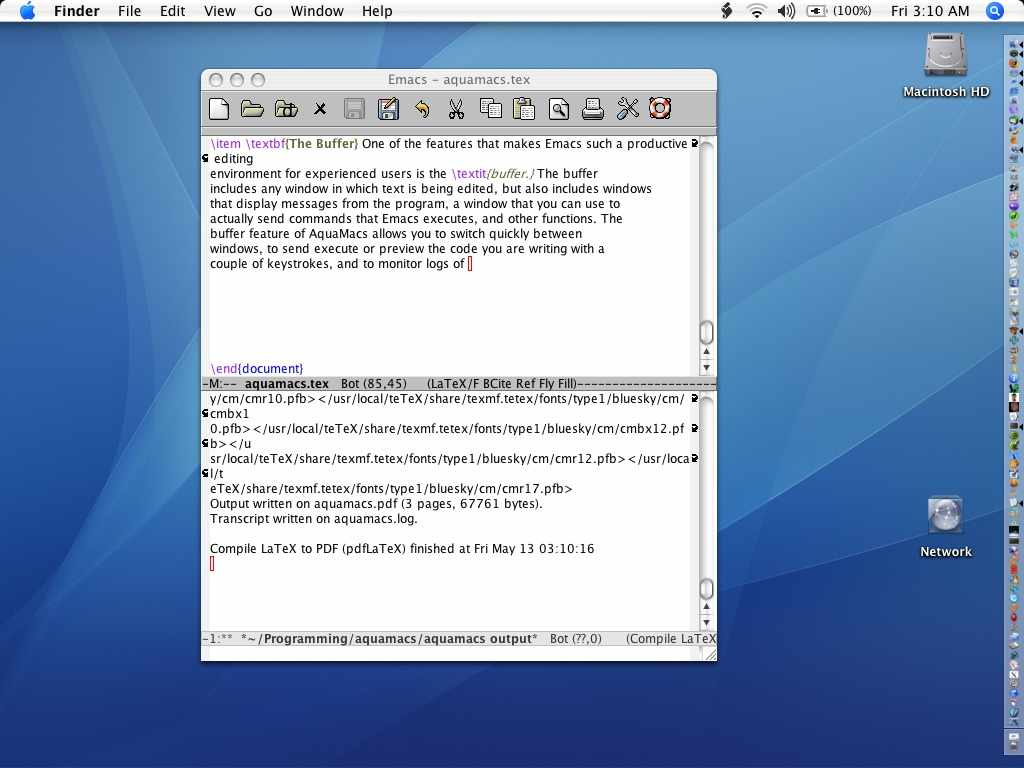
\includegraphics[width=5in]{buffers.jpg}}
\caption{The ``buffer'' feature of Emacs, which Aquamacs preserves, is
a powerful tool for enhancing productivity.}}
\label{buffers.jpg}
\end{figure}

\subsection{Tools}
The Tools menu provides access to a variety of functions, including
integration with version control systems, running shell commands,
searching external files for text, and compiling and debugging
software code. The Tools menu also provides access to newsgroups and
e-mail in a command-line capacity.\footnote{The functionality
provided in the Tools menu is, to say the least, diverse, and is part
of the attraction of Emacs for a large number of users---particularly
advanced users. It is not necessary to use Aquamacs as an e-mail
client to appreciate its considerable power and utility, however.}

\subsection{Help}
The Help menu contains a wealth of information about
Aquamacs/Emacs. Except for the help provided in this document,
Aquamacs' Help menu provides no documentation of the Mac-specific
customizations that you will find in Emacs. However, the general Emacs
user help is comprehensive and detailed to the point of possibly
overwhelming the inexperienced user. The beginner should definitely
start with the Emacs tutorial contained in the Help menu. While geared
toward the traditional Emacs interface instead of the OS X Aquamacs
version, the tutorial is a good introduction to Emacs' unique
capabilities. And, as you gain more experience, you will appreciate
the depth of the Emacs documentation. 

\section{Aquamacs for Emacs Veterans}

While experienced users of Emacs on other platforms can continue to
use all the key combinations to which they are accustomed, we
recommend that they use the Aquamacs-specific conventions to get the
most benefit from the applications.  Many of the
standard Emacs behaviors and interface conventions have been modified
in Aquamacs in the interest of proving a more Aqua-native
experience. In this section, we discuss some of the ways that Emacs
conventions are mapped to Aqua conventions, and outline some advanced ways that users can modify Aquamacs to their specific preferences.

\subsection{Keyboard Shortcuts}
Emacs has a well-defined set of keyboard shortcuts, which Aquamacs
revises to accomodate OS X conventions. See Table \ref{tab:shortcuts}
and Table \ref{tab:command} for details.



\begin{table}[t]
\begin{center}
 \begin{tabular}{|c|c|c|}
\hline  \textbf{Shortcut} &  \textbf{Elisp Command} &   \textbf{Function}\\ 

\hline Apple-N &new-frame-with-new-scratch & Open a new empty window/frame\\

\hline Apple-O & mac-find-file-other-frame & Open a new window/frame with a file\\

\hline Apple-shift-s & mac-save-file-as & Save as\\

\hline Apple-shift-O &find-file-other-frame & Find file in another frame\\

\hline Apple-A & mark-whole-buffer & Select all text\\

\hline Apple-V & yank & Paste text\\

\hline Apple-C & kill-ring-save & Copy text\\

\hline Apple-X &  kill-region & Cut text\\

\hline Apple-S &  save-buffer & Save file\\

\hline Apple-L &  goto-line & Go to specified line\\

\hline Apple-F & isearch-forward & Search\\

\hline Apple-G &  isearch-repeat-forward & Repeat search\\

\hline  Apple-W &  `intelligent-close) & Close window\\

\hline Apple-M & iconify-or-deiconify-frame & Minimize window to the Dock\\

\hline Apple-. & keyboard-quit) & Keyboard quit\\

\hline Apple-Q & `save-buffers-kill-emacs) & Save file, exit program\\

\hline Apple-Z & undo & Undo\\

\hline Apple-shift-Z &  redo & Redo\\

\hline 
\end{tabular} 
\caption{Aqua-specific keyboard shortcuts implemented in Aquamacs.}
\label{tab:shortcuts}
\end{center}
\end{table}


\begin{table}[t]
\begin{center}
 \begin{tabular}{|c|c|}
\hline \textbf{Emacs Command Key} & \textbf{Aqua Command Key}\\
\hline C-* & Control-*\\
\hline H-* & Apple-*\\
\hline A-* & Option-*\\
\hline C-M-* & ESC Control-*\\
\hline 
\end{tabular} 
\caption{Aqua-specific command keys implemented in Aquamacs.}
\label{tab:command}
\end{center}
\end{table}


\subsection{Customizing Aquamacs}
One of the distinguishing features of Emacs is the degree to which it
can be customized by the end user. Emacs includes its own internal
scripting language, elisp, which allows the user to customize such
things as keyboard shortcuts, window settings, fonts, and more. The
Aquamacs customizations themselves are implemented in elisp.\footnote{The Aquamacs
customizations are stored in elisp files in the application bundle. It
is possible to modify these files directly, but we discourage this
practice and provide no support for it.}


We recommend that user customizations be placed in specific
locations. See Table \ref{tab:prefs} for more information.

%\begin{sidewaystable}[t]
\begin{table}[t]
\begin{center}
\begin{tabular}{|c|c|}
\hline  \textbf{Location} & \textbf{Type} \\ 
\hline  /Library/Preferences/Emacs/Preferences &  Preferences
for all  Carbon Emacs installations\\ 
\hline  /Library/Preferences/Aquamacs Emacs/Preferences &
Preferences for Aquamacs and for all users\\ 
\hline  /Users/username/Library/Emacs/Preferences & User-specific preferences for all Carbon Emacs installations \\ 
\hline /Users/username/Library/Aquamacs Emacs/Preferences  &  User-specific preferences for Aquamacs \\ 
\hline 
\end{tabular} 
\caption{Standard locations for Aquamacs user customizations.}
\label{tab:prefs}
\end{center}
%end{sidewaystable}
\end{table}

It is also possible to define and store user
customizations in the traditional .emacs file, which is
placed in the user's home directory. This option is deprecated in
Aquamacs, however.

Below are some specific customization items that may be of interest:

\begin{itemize} 
\item \textbf{Frame.} Aquamacs opens new files (and other buffers) in
  new frames. That is usually more convenient and allows you to use
  the graphical user  interface of today's computers, which did not
  exist when Emacs was  conceived almost three decades ago. If you do
  not like this behavior, perhaps  because you are used to traditional
  Emacs, just deselect  ``Display Buffers in Separate Frames'' in the
  Options menu and save  your choice with ``Save Options.''

\item \textbf{Colors and fonts for frames and modes.} Aquamacs allows
  you to alter specific features of the current frame  via functions
  in the Options menu. ``Set Color Theme...'' will let you choose a
  pre-defined combination  of colors and fonts. ``Set Font...'' gives you a choice of pre-defined fonts to use.

These settings only apply to the current frame. To make them ``stick,'' use the function ``Set current theme as default.'' Then, all  future frames will open with the new colors and fonts chosen. This  applies to all frame-settings that a mode or you as a user have  chosen using Emacs' configuration system. The choice of a default  theme will stick until you restart Aquamacs Emacs.

Aquamacs Emacs also offers you to pick a theme specific to the
current mode. For example, you can use different settings when you are
editing C or LaTeX, then when you are editing a text file. That is
what  the function ``Set current theme for current mode'' is for. Again, the setting  will stick for newly opened frames or or whenever you newly use a  given mode, until you restart Aquamacs Emacs.

Finally, you may want to save your settings so they will stick even
when you restart Aquamacs Emacs. To do so, use the function ``Save Options.''


\begin{figure}
\centering
{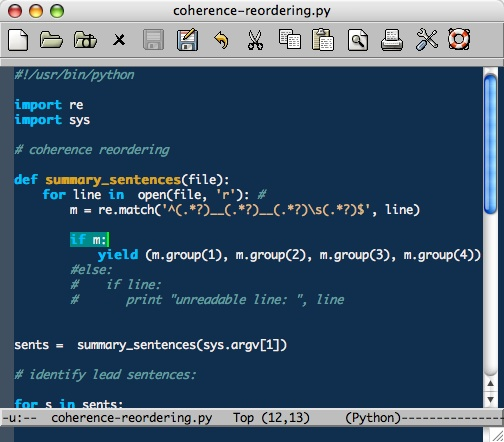
\includegraphics[width=5in]{theme.jpg}}
\caption{Aquamacs with a custom theme applied.}}
\label{theme.jpg}
\end{figure}

\item \textbf{Additional customization.} Of course, Aquamacs Emacs
  offers you almost all the customization  possibilities that Emacs
  has. Under ``Customize Emacs,'' you will find  a sub-menu that
  allows you to browse the vast space of customization
  settings. Beware: some of them are complex and not easy to
  understand. If you would like to tinker with some Aquamacs-specific
  behavior, you can customize the group ``Aquamacs.''

\end{itemize}


The range of possible customizations---including restoring some of
Emacs' traditional interface conventions---is beyond the scope of this
help document. However, we provide a wiki for users to share their
modifications. See
\url{http://www.emacswiki.org/cgi-bin/wiki/AquamacsEmacs/} for more
details. 





\subsection{\LaTeX\ Support}
One special feature of Aquamacs is its extensive support for the
editing of \LaTeX documents, especially Emacs' Auc\TeX\ mode. 

\begin{figure}
\centering
{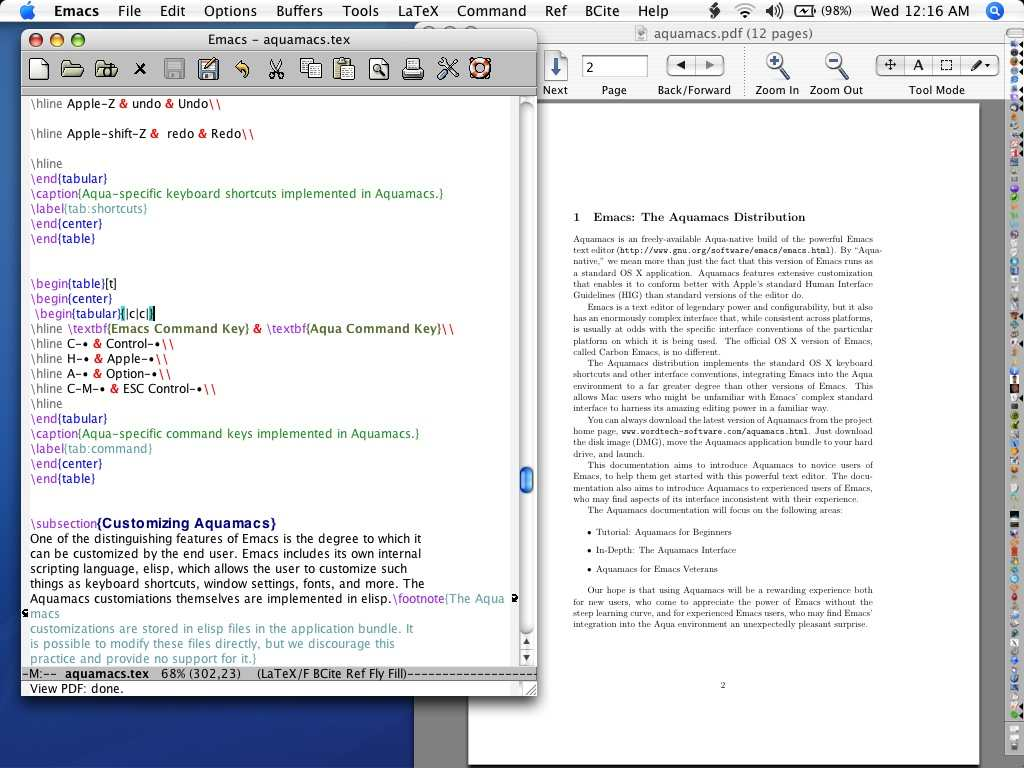
\includegraphics[width=5in]{aquamacs-tex.jpg}}
\caption{Aquamacs offers extensive support for \LaTeX\ documents.}}
\label{aquamacs-tex.jpg}
\end{figure}

The following is necessary to fully access the enhanced \LaTeX\
functionality that Aquamacs offers:

 Install Gerben Wierda's \TeX\ package for Mac OS X. This package
  is the most complete and user-friendly \TeX\ distribution for the
  Mac. You can download the installer package at
  \url{http://www.rna.nl/tex.html}. While you can obtain \TeX\ from
  other sources, only the Gerben Wierda distribution is supported in
  Aquamacs at this time.

 Install the Auc\TeX\ package maintained by Norm Gall. This
  package can be downloaded from
  \url{http://yaced.sourceforge.net}. The installer will give you the
  option to select the installation directory; do not choose the
  default location, but instead pick /Library/Application
  Support/Emacs. (Other locations are not supported in 
  Aquamacs.)\footnote{Norm Gall maintains
  a full distribution of Emacs called Yet Another Carbon Emacs
  Distribution (Yaced) that is a standard build of Emacs on the
  Mac. If you are accustomed to the Emacs interface and prefer not to
  have that interface mapped to OS X conventions, you may want to
  consider using Yaced instead of Aquamacs.}

\section{Getting Help}

There are many options for getting help with Aquamacs.

From within Aquamacs, you can access user documentation from the menu
or from specific key combinations: c-h k (key/menu entry) brings up
help for some input items; C-h f (function) gives help for an elisp
function; autocompletion support is available with (tab); and  
c-h a brings up apropos, a search function.

For help from other Aquamacs/Emacs users, the best place
to begin is the OS X Emacs mailing
list. The searchable list archives are located at
\url{http://www.esm.psu.edu/mac-tex/MacOSX-Emacs-Digests/}. For more
information on subscribing to the list, see
\url{http://www.aquamacs.org}.

Another option for general Emacs help is the gnu.emacs.help newsgroup.

In addition to requesting help, you can also offer it. Apart from
answering questions at the OS X Emacs mailing list, you can also file
bug reports on Aquamacs. Use the ``Send Bug Report" function in the
Help menu  (general Emacs bugs, too), and also our Aquamacs-specific
bug report  system at \url{http://sourceforge.net/projects/aquamacs}. 


\section{Acknowledgments}


We would also like to acknowledge the contributions of these authors, whose source code and hints on public forums have already been integrated into the build:
Andrew Choi (main Emacs-to-Mac port);  Drew Adams;
Lawrence Akka;
 Emil Astrom; 
Stefan Bruda; 
Steve Dodd; 
Massimiliano Gubinelli (Emacs icon); 
 Kyle E. Jones; 
 Pekka Marjola;
Yamamoto Mitsuharu;
Gerd Neugebauer;
 Ovidiu Predesc; 
Steven Tamm;
 Bob Weiner;  
Milan Zamazal; and 
Seiji Zenitani.

Emacs is the work of Richard Stallman and many other developers.

\section {Licenses}

Aquamacs: the Emacs distribution, (c) 2005 by David Reitter, Kevin
Walzer and individual contributors. Aquamacs is licensed under the terms of the GNU General Public License. For details of this license, please see \url{http://www.gnu.org/copyleft/gpl.html}. The Aquamacs documentation is licensed under the terms of the GNU Free Documentation License. For details of this license, please see \url{http://www.gnu.org/copyleft/fdl.html#SEC1}.
\end{document}